\documentclass[]{article}
\usepackage{lmodern}
\usepackage{amssymb,amsmath}
\usepackage{ifxetex,ifluatex}
\usepackage{fixltx2e} % provides \textsubscript
\ifnum 0\ifxetex 1\fi\ifluatex 1\fi=0 % if pdftex
  \usepackage[T1]{fontenc}
  \usepackage[utf8]{inputenc}
\else % if luatex or xelatex
  \ifxetex
    \usepackage{mathspec}
  \else
    \usepackage{fontspec}
  \fi
  \defaultfontfeatures{Ligatures=TeX,Scale=MatchLowercase}
\fi
% use upquote if available, for straight quotes in verbatim environments
\IfFileExists{upquote.sty}{\usepackage{upquote}}{}
% use microtype if available
\IfFileExists{microtype.sty}{%
\usepackage{microtype}
\UseMicrotypeSet[protrusion]{basicmath} % disable protrusion for tt fonts
}{}
\usepackage[margin=1in]{geometry}
\usepackage{hyperref}
\hypersetup{unicode=true,
            pdftitle={Report},
            pdfauthor={Drunken Master 2},
            pdfborder={0 0 0},
            breaklinks=true}
\urlstyle{same}  % don't use monospace font for urls
\usepackage{color}
\usepackage{fancyvrb}
\newcommand{\VerbBar}{|}
\newcommand{\VERB}{\Verb[commandchars=\\\{\}]}
\DefineVerbatimEnvironment{Highlighting}{Verbatim}{commandchars=\\\{\}}
% Add ',fontsize=\small' for more characters per line
\usepackage{framed}
\definecolor{shadecolor}{RGB}{248,248,248}
\newenvironment{Shaded}{\begin{snugshade}}{\end{snugshade}}
\newcommand{\KeywordTok}[1]{\textcolor[rgb]{0.13,0.29,0.53}{\textbf{#1}}}
\newcommand{\DataTypeTok}[1]{\textcolor[rgb]{0.13,0.29,0.53}{#1}}
\newcommand{\DecValTok}[1]{\textcolor[rgb]{0.00,0.00,0.81}{#1}}
\newcommand{\BaseNTok}[1]{\textcolor[rgb]{0.00,0.00,0.81}{#1}}
\newcommand{\FloatTok}[1]{\textcolor[rgb]{0.00,0.00,0.81}{#1}}
\newcommand{\ConstantTok}[1]{\textcolor[rgb]{0.00,0.00,0.00}{#1}}
\newcommand{\CharTok}[1]{\textcolor[rgb]{0.31,0.60,0.02}{#1}}
\newcommand{\SpecialCharTok}[1]{\textcolor[rgb]{0.00,0.00,0.00}{#1}}
\newcommand{\StringTok}[1]{\textcolor[rgb]{0.31,0.60,0.02}{#1}}
\newcommand{\VerbatimStringTok}[1]{\textcolor[rgb]{0.31,0.60,0.02}{#1}}
\newcommand{\SpecialStringTok}[1]{\textcolor[rgb]{0.31,0.60,0.02}{#1}}
\newcommand{\ImportTok}[1]{#1}
\newcommand{\CommentTok}[1]{\textcolor[rgb]{0.56,0.35,0.01}{\textit{#1}}}
\newcommand{\DocumentationTok}[1]{\textcolor[rgb]{0.56,0.35,0.01}{\textbf{\textit{#1}}}}
\newcommand{\AnnotationTok}[1]{\textcolor[rgb]{0.56,0.35,0.01}{\textbf{\textit{#1}}}}
\newcommand{\CommentVarTok}[1]{\textcolor[rgb]{0.56,0.35,0.01}{\textbf{\textit{#1}}}}
\newcommand{\OtherTok}[1]{\textcolor[rgb]{0.56,0.35,0.01}{#1}}
\newcommand{\FunctionTok}[1]{\textcolor[rgb]{0.00,0.00,0.00}{#1}}
\newcommand{\VariableTok}[1]{\textcolor[rgb]{0.00,0.00,0.00}{#1}}
\newcommand{\ControlFlowTok}[1]{\textcolor[rgb]{0.13,0.29,0.53}{\textbf{#1}}}
\newcommand{\OperatorTok}[1]{\textcolor[rgb]{0.81,0.36,0.00}{\textbf{#1}}}
\newcommand{\BuiltInTok}[1]{#1}
\newcommand{\ExtensionTok}[1]{#1}
\newcommand{\PreprocessorTok}[1]{\textcolor[rgb]{0.56,0.35,0.01}{\textit{#1}}}
\newcommand{\AttributeTok}[1]{\textcolor[rgb]{0.77,0.63,0.00}{#1}}
\newcommand{\RegionMarkerTok}[1]{#1}
\newcommand{\InformationTok}[1]{\textcolor[rgb]{0.56,0.35,0.01}{\textbf{\textit{#1}}}}
\newcommand{\WarningTok}[1]{\textcolor[rgb]{0.56,0.35,0.01}{\textbf{\textit{#1}}}}
\newcommand{\AlertTok}[1]{\textcolor[rgb]{0.94,0.16,0.16}{#1}}
\newcommand{\ErrorTok}[1]{\textcolor[rgb]{0.64,0.00,0.00}{\textbf{#1}}}
\newcommand{\NormalTok}[1]{#1}
\usepackage{longtable,booktabs}
\usepackage{graphicx,grffile}
\makeatletter
\def\maxwidth{\ifdim\Gin@nat@width>\linewidth\linewidth\else\Gin@nat@width\fi}
\def\maxheight{\ifdim\Gin@nat@height>\textheight\textheight\else\Gin@nat@height\fi}
\makeatother
% Scale images if necessary, so that they will not overflow the page
% margins by default, and it is still possible to overwrite the defaults
% using explicit options in \includegraphics[width, height, ...]{}
\setkeys{Gin}{width=\maxwidth,height=\maxheight,keepaspectratio}
\IfFileExists{parskip.sty}{%
\usepackage{parskip}
}{% else
\setlength{\parindent}{0pt}
\setlength{\parskip}{6pt plus 2pt minus 1pt}
}
\setlength{\emergencystretch}{3em}  % prevent overfull lines
\providecommand{\tightlist}{%
  \setlength{\itemsep}{0pt}\setlength{\parskip}{0pt}}
\setcounter{secnumdepth}{0}
% Redefines (sub)paragraphs to behave more like sections
\ifx\paragraph\undefined\else
\let\oldparagraph\paragraph
\renewcommand{\paragraph}[1]{\oldparagraph{#1}\mbox{}}
\fi
\ifx\subparagraph\undefined\else
\let\oldsubparagraph\subparagraph
\renewcommand{\subparagraph}[1]{\oldsubparagraph{#1}\mbox{}}
\fi

%%% Use protect on footnotes to avoid problems with footnotes in titles
\let\rmarkdownfootnote\footnote%
\def\footnote{\protect\rmarkdownfootnote}

%%% Change title format to be more compact
\usepackage{titling}

% Create subtitle command for use in maketitle
\newcommand{\subtitle}[1]{
  \posttitle{
    \begin{center}\large#1\end{center}
    }
}

\setlength{\droptitle}{-2em}

  \title{Report}
    \pretitle{\vspace{\droptitle}\centering\huge}
  \posttitle{\par}
    \author{Drunken Master 2}
    \preauthor{\centering\large\emph}
  \postauthor{\par}
      \predate{\centering\large\emph}
  \postdate{\par}
    \date{Due 5 November 2018}


\begin{document}
\maketitle

{
\setcounter{tocdepth}{3}
\tableofcontents
}
\subsection{Introduction}\label{introduction}

Bootstrapping is an area of statistics that is usually implemented using
simple Monte Carlo simulations whereby a certain calculation is repeated
a large number of times with random sampling (ref?). Repeating
calculations a large number of times, say 1,000,000 times, can become
slow to compute. Therefore, the use of efficient and fast code is
essential.

This is project aimed to improve and produce two fast and efficient
bootstrap functions using R 3.5.1 (R, 2018) and SAS 9.4 (SAS Institute,
Cary NC).

\begin{Shaded}
\begin{Highlighting}[]
\NormalTok{fitData <-}\StringTok{ }\KeywordTok{read.csv}\NormalTok{(}\StringTok{"data/fitness.csv"}\NormalTok{)}
\end{Highlighting}
\end{Shaded}

A short example analysis was given for each function. The fitness
dataset from Rawlings (1998) contains measurements of the following
seven variables obtained from 31 men: • Age: Age in years • Weight:
Weight in kg • Oxygen: Oxygen intake rate, ml per kg body weight per
minute • RunTime: time to run 1.5 miles in minutes • RestPulse: heart
rate while resting • RunPulse: heart rate at end of run • MaxPulse:
maximum heart rate recorded while running All alnalyses in the following
report were carried out using R 3.5.1 software.

\pagebreak

\subsection{R}\label{r}

\subsubsection{\texorpdfstring{\emph{The function
lmBoot}}{The function lmBoot}}\label{the-function-lmboot}

The function \emph{lmBoot} (Appendix A.\#\#\#) uses bootstrap sampling
methods to calculate estimates for the means and confidence intervals of
the slope and intercept parameters produced by a linear regression.

The function takes in two arguments:

\begin{itemize}
\tightlist
\item
  inputData: the dataset that will be used for sampling, where the
  response variable is in the first column and the remainder of the
  columns contain the covariates of interest.
\item
  nBoot: The number of bootstrap samples to compute.
\end{itemize}

The function outputs:

\begin{itemize}
\tightlist
\item
  BootResults: An array with the number of rows equivalent to the nBoot
  argument and as many columns as there are Beta coeficients; i.e.~for
  the intercept and covariates.
\item
  ConfidenceIntervals: A matrix containing 95\% confidence intervals for
  each parameter estimate.
\end{itemize}

\subsubsection{\texorpdfstring{\emph{Changes made to
lmBoot}}{Changes made to lmBoot}}\label{changes-made-to-lmboot}

\begin{enumerate}
\def\labelenumi{\arabic{enumi}.}
\item
  The original lmBoot function only produced bootstrap samples for one
  covariate. This was changed so that lmBoot\_2 produces bootstrap
  estimates for a multiple number of covariates and calculates
  confidence intervals for each parameter estimate.
\item
  The use of the \emph{lm} function was removed and the beta
  coefficients were calculated using matrix calculations instead.
\end{enumerate}

\[
\beta = (X^TX)^{-1}X^TY
\]

\begin{enumerate}
\def\labelenumi{\arabic{enumi}.}
\setcounter{enumi}{2}
\item
  \emph{forloops} are relatively slow and inefficient. Therefore, the
  \emph{forloop} was replaced using \emph{sapply} which applies a
  function to each element of a matrix. The function called
  \emph{bootLM} was written to carry out the bootstrap algorithm.
\item
  Parallelisation
\end{enumerate}

Table \#\#\# illustrates differences in runtime for three different
versions of the lmBoot function; the original, an improved version and a
parallelised version. Each function was timed on how long it took to
resample 100, 1000, 10000 and 100000 samples.

\begin{longtable}[]{@{}llll@{}}
\caption{Changes in Runtime (in seconds) of lmBoot}\tabularnewline
\toprule
Samples & lmBoot & lmBoot Improved & lmBoot Parallised\tabularnewline
\midrule
\endfirsthead
\toprule
Samples & lmBoot & lmBoot Improved & lmBoot Parallised\tabularnewline
\midrule
\endhead
100 & 0.079 & 0.006 & 0.02\tabularnewline
1000 & 0.941 & 0.052 & 0.026\tabularnewline
10000 & 8.502 & 0.564 & 0.052\tabularnewline
100000 & - & 5.538 & 0.37\tabularnewline
\bottomrule
\end{longtable}

\subsubsection{\texorpdfstring{\emph{Example analysis using
lmBoot}}{Example analysis using lmBoot}}\label{example-analysis-using-lmboot}

\begin{verbatim}
## Loading required package: foreach
\end{verbatim}

\begin{verbatim}
## Loading required package: iterators
\end{verbatim}

\begin{verbatim}
## Loading required package: parallel
\end{verbatim}

\begin{verbatim}
## 
## Attaching package: 'dplyr'
\end{verbatim}

\begin{verbatim}
## The following objects are masked from 'package:stats':
## 
##     filter, lag
\end{verbatim}

\begin{verbatim}
## The following objects are masked from 'package:base':
## 
##     intersect, setdiff, setequal, union
\end{verbatim}

\begin{longtable}[]{@{}lrr@{}}
\caption{95\% Confidence Intervals}\tabularnewline
\toprule
& 2.5\% & 97.5\%\tabularnewline
\midrule
\endfirsthead
\toprule
& 2.5\% & 97.5\%\tabularnewline
\midrule
\endhead
Intercept & 78.864 & 121.256\tabularnewline
Age & -0.425 & -0.005\tabularnewline
Weight & -0.159 & 0.062\tabularnewline
RunTime & -3.295 & -1.854\tabularnewline
RestPulse & -0.181 & 0.102\tabularnewline
RunPulse & -0.565 & -0.091\tabularnewline
MaxPulse & -0.030 & 0.527\tabularnewline
\bottomrule
\end{longtable}

\begin{figure}
\centering
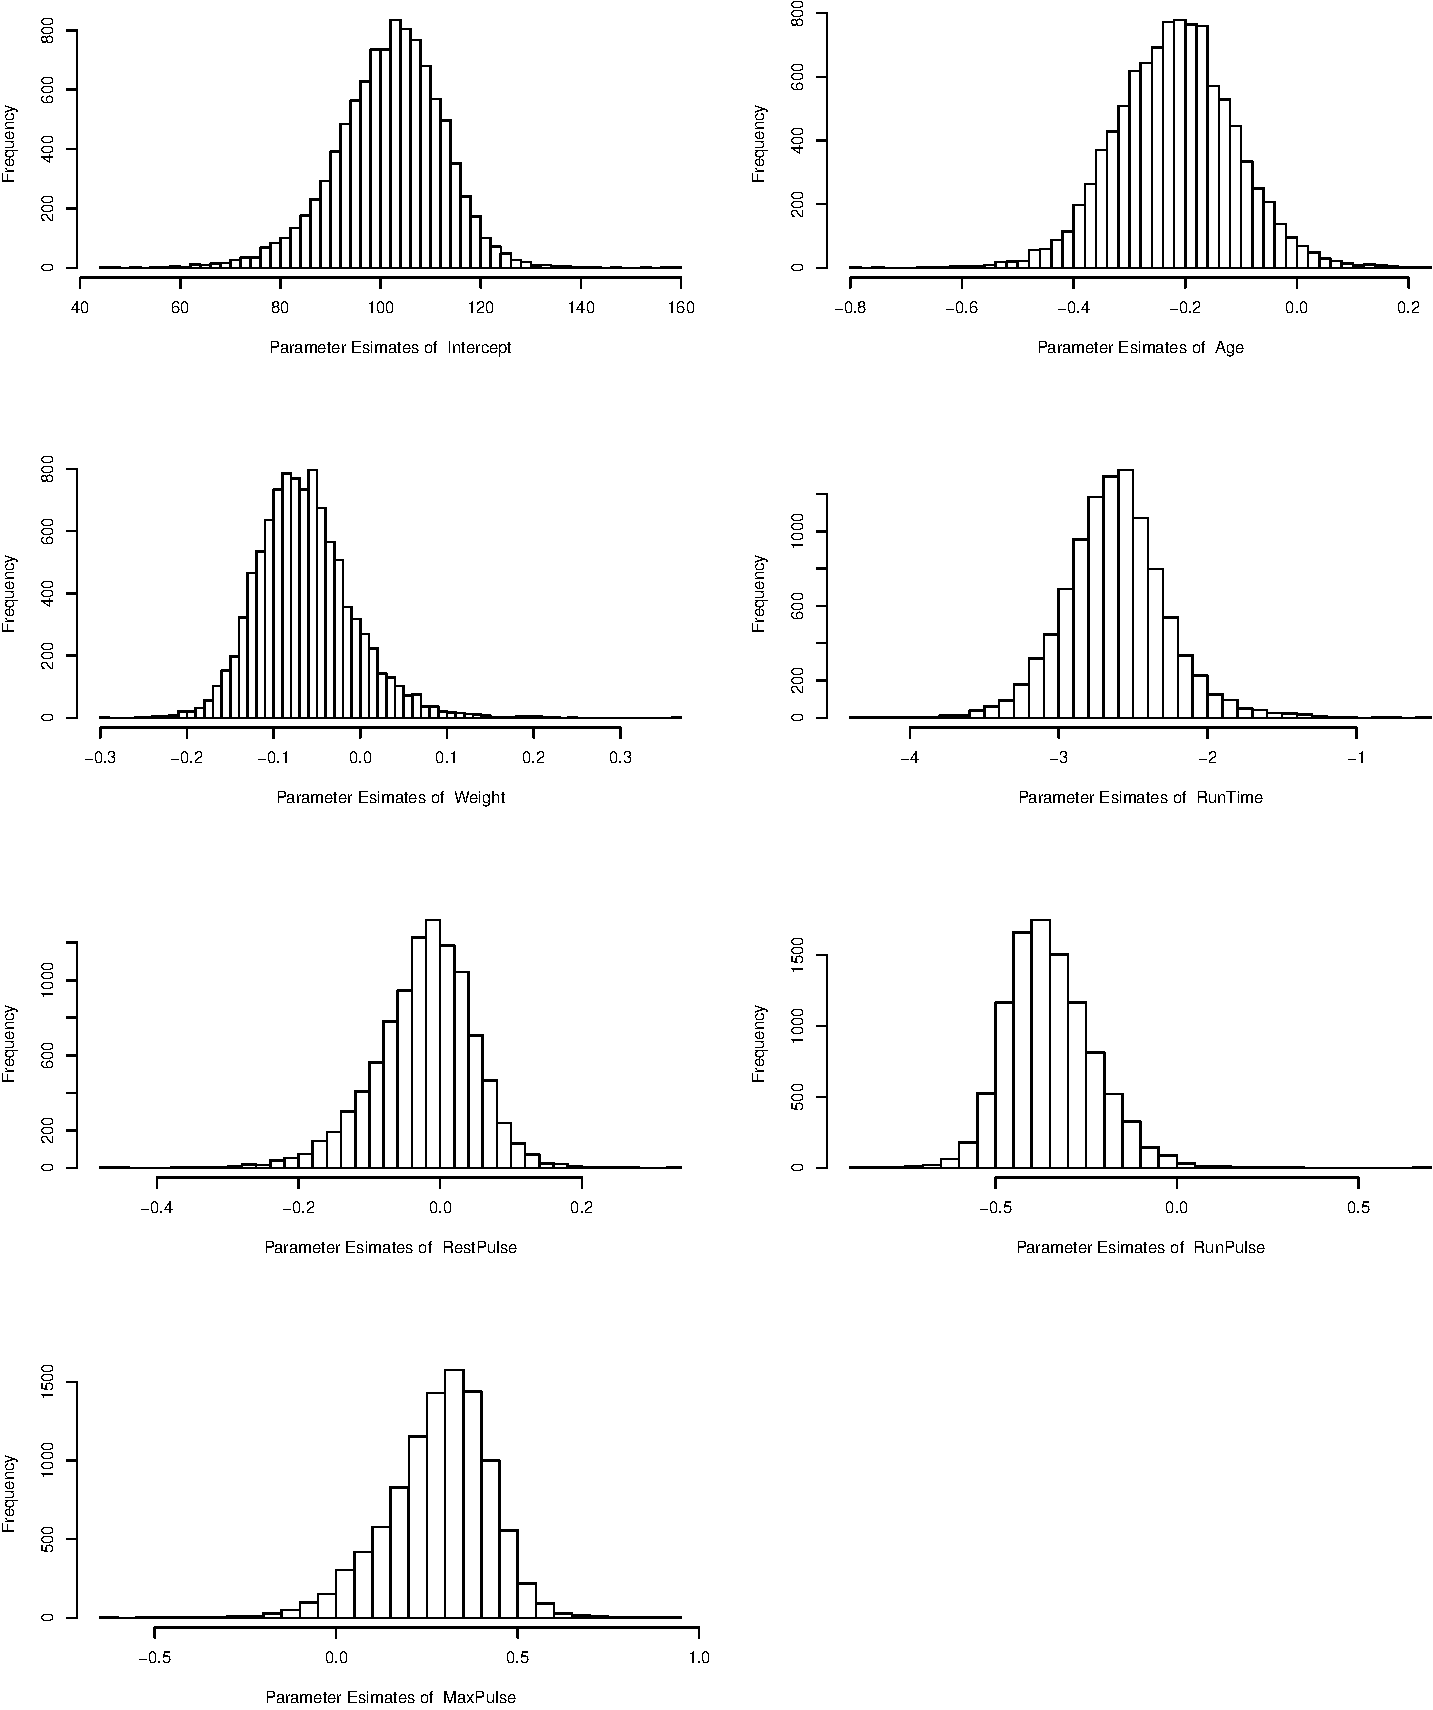
\includegraphics{Report_files/figure-latex/rcode-1.pdf}
\caption{\label{fig:rcode} Bootstrap Distributions of Parameter
Estimates}
\end{figure}

\pagebreak 

\subsection{SAS}\label{sas}

\subsubsection{\texorpdfstring{\emph{The program
SASBoot}}{The program SASBoot}}\label{the-program-sasboot}

The macro program \emph{SASBoot} (Appendix A.\#\#\#) uses bootstrap
sampling methods to calculate estimates for the means and confidence
intervals of the slope and intercept parameters produced by a linear
regression.

It takes in four agruments:

\begin{itemize}
\tightlist
\item
  NumberOfLoops: the number of bootstrap iterations.
\item
  DataSet: A SAS dataset containing the response and covariate.
\item
  XVariable: The covariate for our regression model (gen. continuous
  numeric).
\item
  YVariable: The response variable for our regression model (gen.
  continuous numeric).
\end{itemize}

The program then outputs:

\begin{itemize}
\tightlist
\item
  ResultHolder: A SAS dataset with the number of rows equivalent to the
  NumberOfLoops argument and two columns; RandomIntercept and
  RandomSlope.
\item
  output.rtf: An RTF file containing 95\% confidence intervals for the
  mean, the mean estimate for each parameter and plots of the
  distributions of the bootstrap parameters.
\end{itemize}

The function makes use of:

\begin{itemize}
\tightlist
\item
  MACRO statements to create a flexible program with input arguments.
\item
  PROC SURVEYSELECT which allows the use of random sampling to generate
  random samples from a selected or inputed dataset.
\item
  PROC REG to perform a linear regression.
\end{itemize}

\subsubsection{\texorpdfstring{\emph{Changes made to
SASBoot}}{Changes made to SASBoot}}\label{changes-made-to-sasboot}

The changes made to SASBoot were motivated, in part, by the work of
Cassel (2018) in his paper ``Don't Be Loopy: Re-Sampling and Simulation
the SAS® Way''.

\begin{enumerate}
\def\labelenumi{\arabic{enumi}.}
\tightlist
\item
  The \%do\% loop was first removed and the following code was added to
  PROC SURVEYSELECT:\\
  \emph{samprate = 1}\\
  \emph{outhits}\\
  \emph{rep = \&NumberOfLoops}
\end{enumerate}

which ensures that NumberOfLoops samples of the same size as the
original data set are produced and recorded.

\begin{enumerate}
\def\labelenumi{\arabic{enumi}.}
\setcounter{enumi}{1}
\item
  A linear regression using PROC REG was improved by introducing the
  by-variable REPLICATE. This variable is automatically produced from
  PROC SURVEYSELECT to keep track of each new bootstrap sample, and
  ensures that the linear regression is run on each sample. Thus, only
  the Result Holder Dataset was necessary, and there was no need to
  generate the Temp Dataset.
\item
  The SASFILE statement was included to upload the dataset to RAM rather
  than the hard drive before any sampling was carried out so that the
  dataset does not have to be read-in every time a resample is done.
\end{enumerate}

(4. Replaced noprint and ODS listing close - still working on this)

The program was run six times and Table \#\#\# displays the runtime (in
seconds) for 1000 loops. The code used to measure the run time of the
SASBoot program can be found in Appendix A.\#\#\# (H, 2012).

\begin{longtable}[]{@{}rcr@{}}
\caption{Changes in Runtime of SASBoot}\tabularnewline
\toprule
RegBoot & SASBoot & SASBoot (with rtf output)\tabularnewline
\midrule
\endfirsthead
\toprule
RegBoot & SASBoot & SASBoot (with rtf output)\tabularnewline
\midrule
\endhead
183.360 & 0.297 & 6.068\tabularnewline
189.973 & 6.087 & 6.087\tabularnewline
195.420 & 0.422 & 6.064\tabularnewline
192.835 & 0.313 & 6.041\tabularnewline
192.786 & 0.296 & 5.941\tabularnewline
193.558 & 0.314 & 6.062\tabularnewline
\bottomrule
\end{longtable}

\subsubsection{\texorpdfstring{\emph{Example analysis using
SASBoot}}{Example analysis using SASBoot}}\label{example-analysis-using-sasboot}

\begin{Shaded}
\begin{Highlighting}[]
\CommentTok{#Include plots and interpretation}
\end{Highlighting}
\end{Shaded}

An example analysis was conducted using the fitness datset. A linear
model was set up with Oygen as the response and Weight as the covariate.
The bootstrap 95\% confidence intervals produced by SASBoot were then
used to test the null hypothesis that there is no relationship between
Oxygen and Weight, i.e. \(\beta_i = 0\).

If the confidence interval contains 0, one then fails to reject the null
hypothesis and if it does not contain 0 one can reject the null
hypothesis.

The confidence interval for the intercept term (36.4824, 73.1590) does
not contain 0 which suggests that the estimator is not signicant at the
5\% level. The confidence interval for the intercept term (-0.32842,
0.13533) does contain 0 which suggests that the estimator is signicant
at the 5\% level.

\pagebreak 

\subsection{References}\label{references}

Cassell, D. (2018). Don't Be Loopy: Re-Sampling and Simulation the SAS®
Way. {[}online{]}. Available at:
\url{http://www2.sas.com/proceedings/forum2007/183-2007.pdf} {[}Accessed
26 Oct. 2018{]}.

Donovan, C. (2018). MT5763 Project 2 - code collaboration and computer
intensive inference. {[}Online{]}.

H, J. (2012). To calculate SAS program run time. {[}online{]}. Available
at:
\url{http://sashowto.blogspot.com/2012/06/to-calculate-sas-program-run-time.html}
{[}Accessed 26 Oct. 2018{]}.

R Core Team (2018). R: A language and environment for statistical
computing. R Foundation for Statistical Computing, Vienna, Austria.
Available at: \url{https://www.R-project.org/}.

SAS 9.4, SAS Institute Inc., Cary, NC, USA.

SAS Institute Inc. 2004. Proceedings of the Twenty-Ninth Annual SAS®
Users Group International Conference. Cary, NC: SAS Institute Inc.

\pagebreak 

\subsection{Appendix}\label{appendix}

\subsubsection{A.\#\#\# The lmBoot
Function}\label{a.-the-lmboot-function}

\begin{Shaded}
\begin{Highlighting}[]
\CommentTok{#The final code used for lmBoot}
\end{Highlighting}
\end{Shaded}

\subsubsection{A.\#\#\# Code to measure program runtime in
SAS}\label{a.-code-to-measure-program-runtime-in-sas}

\begin{Shaded}
\begin{Highlighting}[]
\OperatorTok\KeywordTok{sysfunc}\NormalTok{(}\KeywordTok{datetime}\NormalTok{());}

\NormalTok{  Program of interest to be timed}

\OperatorTok\KeywordTok{sysfunc}\NormalTok{(}\KeywordTok{datetime}\NormalTok{());  }
\OperatorTok\KeywordTok{sysfunc}\NormalTok{(}\KeywordTok{putn}\NormalTok{(}\OperatorTok{&}\NormalTok{_edtm }\OperatorTok{-}\StringTok{ }\ErrorTok{&}\NormalTok{_sdtm, }\FloatTok{12.4}\NormalTok{));  }
\NormalTok{%put It took }\OperatorTok{&}\NormalTok{_runtm seconds to run the program;}
\end{Highlighting}
\end{Shaded}

\subsubsection{A.\#\#\# The SASBoot
Program}\label{a.-the-sasboot-program}

\begin{Shaded}
\begin{Highlighting}[]
\CommentTok{#The final code used for SASBoot}
\end{Highlighting}
\end{Shaded}


\end{document}
